\documentclass{article}

\title{Matplotlib Reference}
\author{Jedediyah Williams}
\date{August 2026}

\usepackage{amsmath}
\usepackage{fancyhdr}
\usepackage[top=2.5cm, bottom=2.3cm, left=1cm, right=1cm]{geometry}
\usepackage{graphicx}
\usepackage{listings}
\usepackage{multicol}
\usepackage{upquote}
\usepackage{xcolor}


% --------------------------------------------------
% Colors
% --------------------------------------------------
\definecolor{codegray}{RGB}{245,245,245}
\definecolor{codeblue}{RGB}{30,80,150}
\definecolor{keyword}{RGB}{120,50,130}
\definecolor{comment}{RGB}{90,120,90}

% --------------------------------------------------
% Code formatting
% --------------------------------------------------
\lstset{
    language=Python,
    basicstyle=\ttfamily\footnotesize,
    backgroundcolor=\color{codegray},
    frame=single,
    rulecolor=\color{gray!30},
    columns=fullflexible,
    keepspaces=true,
    showstringspaces=false,
    keywordstyle=\color{keyword},
    commentstyle=\color{comment},
    stringstyle=\color{codeblue},
    xleftmargin=3pt,
    xrightmargin=3pt,
    aboveskip=3pt,
    belowskip=3pt
}


% --------------------------------------------------
% Header / footer
% --------------------------------------------------
\pagestyle{fancy}
\fancyhf{}
\lhead{\textbf{Matplotlib Reference}}
\rhead{numericalcomputing.net}
\cfoot{}


\begin{document}
\begin{multicols}{2}

\section*{Line and Scatter Plots}
Graphs are fundamental tools for inspecting and communicating with data.
Start by importing the \texttt{pyplot} plotting library: 
\begin{lstlisting}
import matplotlib.pyplot as plt
\end{lstlisting}

\begin{lstlisting}
t = [ 0,  1,   2,   3,   4,   5,   6]   # Time in hours
d = [ 0, 42, 101, 132, 138, 190, 218]   # Distance in miles

plt.plot(t,d)

plt.xlabel('Time (hours)')
plt.ylabel('Distance (miles)')
plt.title('Road Trip Progress')
plt.show()
\end{lstlisting}

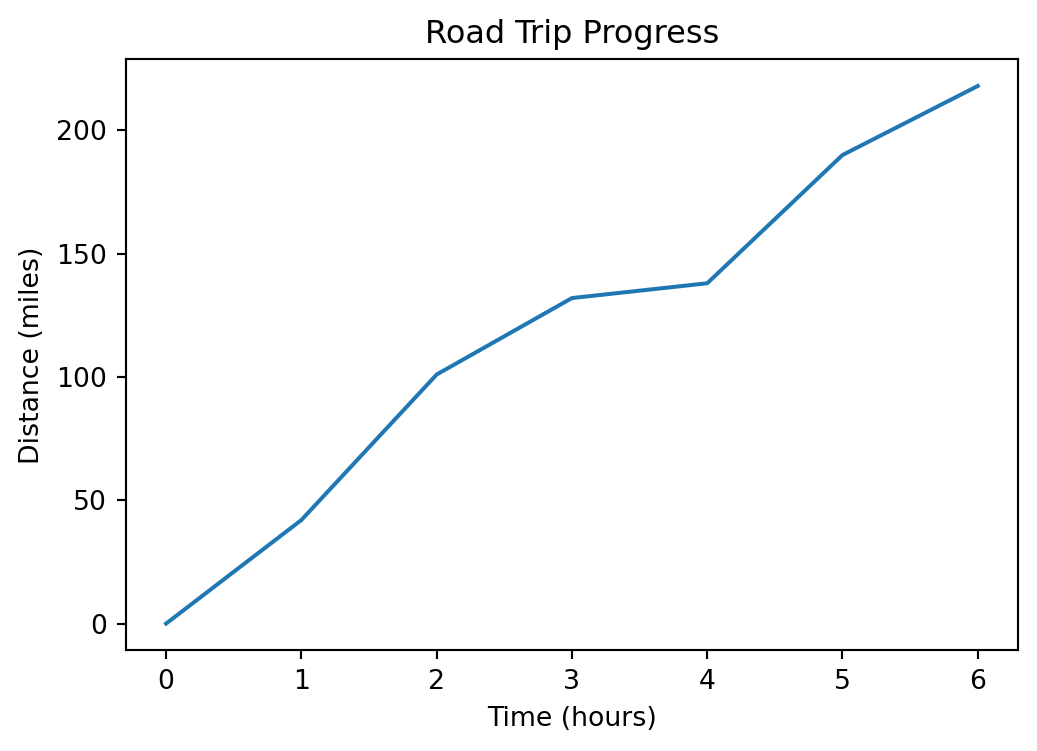
\includegraphics[width=0.45\textwidth]{img/plot_line.png}


\begin{lstlisting}
# Weight in pounds, price in dollars
w = [ 2840, 2900, 3000, 2950, 3150, 3200, 
                   3700, 3900, 3650, 3950]
p = [ 22000, 23500, 21000, 21500, 26000, 
        27000, 31000, 34000, 39000, 44000]

plt.scatter(w,p)

plt.xlabel('Weight (lb)')
plt.ylabel('Price (dollars)')
plt.title('Price per weight of common vehicles')
plt.show() 
\end{lstlisting}
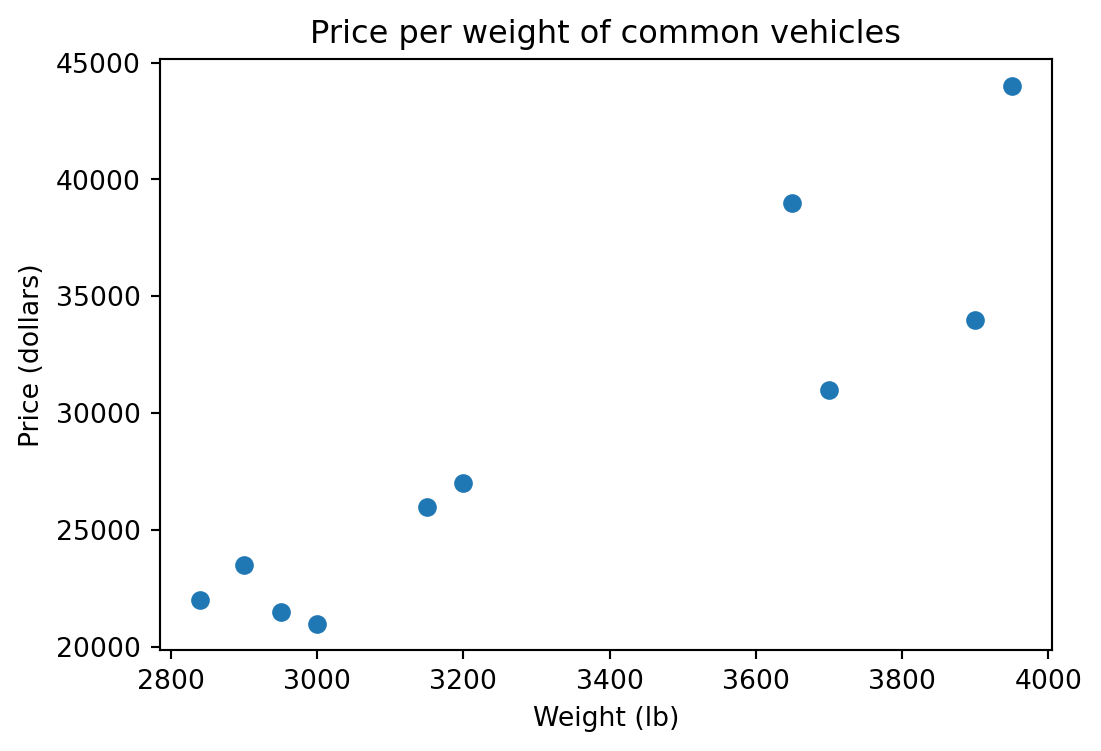
\includegraphics[width=0.45\textwidth]{img/plot_scatter.png}

%A \emph{legend} requires that we \emph{label} the data. 
\begin{lstlisting}
# Data
year = [1800, 1830, 1880, 1900, 1920, 1990, 2000]
Boston = [24937, 61392, 362839, 560862, 748060, 874283, 589141]
NewYork = [60000, 185000, 1919000, 3802000, 
                7798000, 16044000, 17800000]

# Plot both populations
plt.plot(year, Boston, label='Boston') 
plt.plot(year, NewYork, label='New York')

# Display with labels 
plt.xlabel('Year')
plt.ylabel('Population')
plt.title('City Populations')
plt.grid()
plt.legend()
plt.show() 
\end{lstlisting}
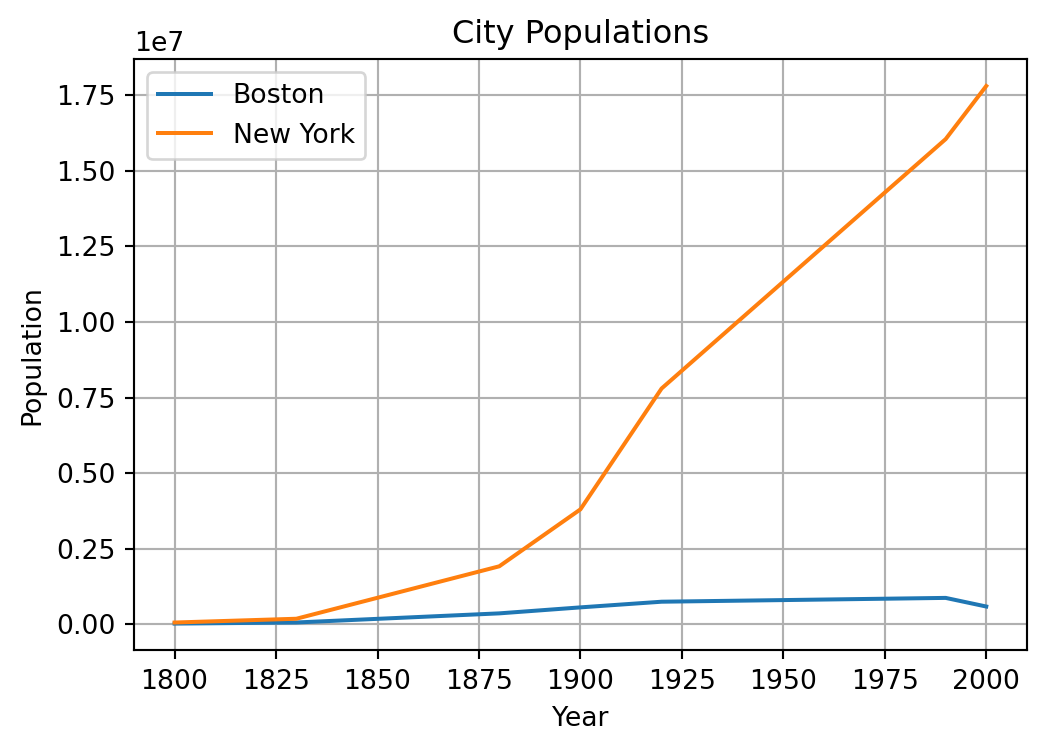
\includegraphics[width=0.4\textwidth]{img/plot_populations.png}

\vspace*{-6mm}
\section*{Plotting with Style}
\begin{lstlisting}
x = [1, 2, 3, 4]
y = [2, 4, 3, 5]

plt.plot( x, y, 
          linestyle='-.',
          marker='o',
          markeredgecolor='red', 
          markerfacecolor='orange',
          markersize=10
         )
plt.show()
\end{lstlisting}

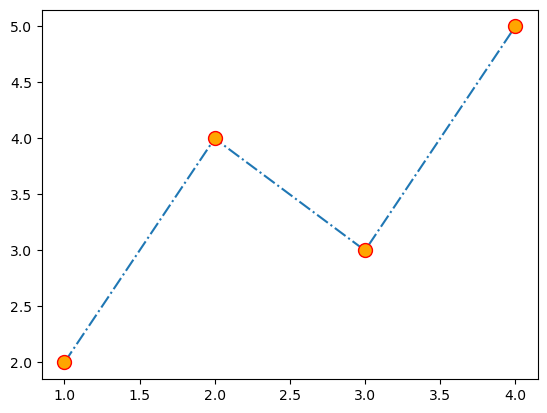
\includegraphics[width=0.35\textwidth]{img/plot_with_style.png}
\\
Marker styles: \texttt{`.'}, \texttt{`*'}, \texttt{`+'}, \texttt{`x'}, \texttt{`o'}, \texttt{`s'} \\ 
Line styles: \texttt{`-'}, \texttt{`--'}, \texttt{`-.'}, \texttt{`:'}, \texttt{`'}

%%%%%%%%%%%%%%%%%%%%%%%%%%%%%%%%%%%%%%%%%
\newpage 


\section*{Bar Chart}

\begin{lstlisting}
study_methods = ['Flashcards', 'ChatBot', 'YouTube', 
                               'Group Study', 'Notes']
counts = [3, 8, 5, 19, 8]

plt.bar(study_methods, counts)
plt.show()
\end{lstlisting}
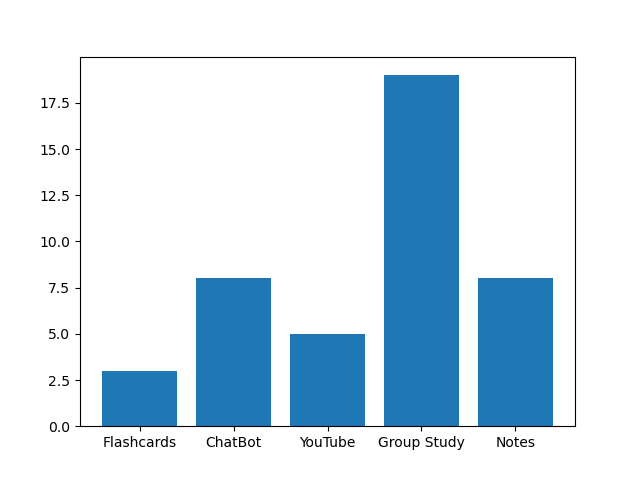
\includegraphics[width=0.45\textwidth]{img/study_bar.png}

\section*{Plotting Distributions}

\begin{lstlisting}
scores = [ 2, 3, 4, 4, 5, 5, 5, 6, 6, 7, 
           7, 7, 8, 8, 8, 8, 9, 9, 10, 10 ]
           
plt.hist(scores, bins=9, edgecolor='black')

plt.xlabel('Score out of 10')
plt.title('Quiz Score Distribution')
plt.show()
\end{lstlisting}

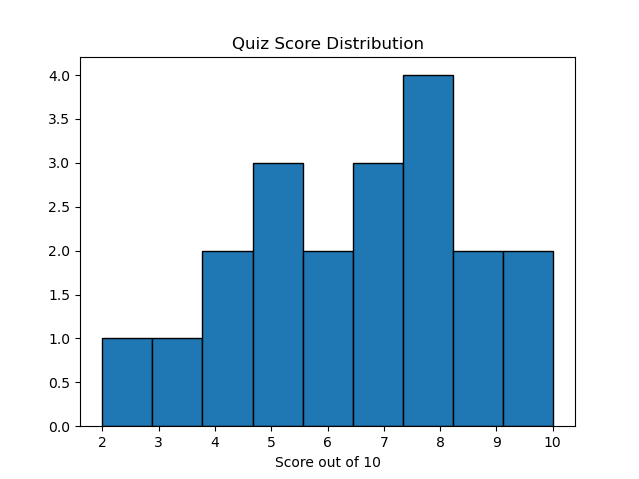
\includegraphics[width=0.45\textwidth]{img/quiz_distribution.png}


Without specifying, the default number of bins in a histogram is 10 and there is no edge color. 


\begin{lstlisting}
class_A = [5, 6, 5, 7, 6, 5, 8, 6, 7, 5, 4, 6, 7, 5, 6]
class_B = [9, 8, 10, 9, 10, 8, 9, 10, 6, 8, 9, 7, 8, 10, 9]

plt.hist(class_A, alpha=0.7, bins=9, label='Class A')
plt.hist(class_B, alpha=0.7, bins=9, label='Class B')

plt.legend()
plt.xlabel('Score out of 10')
plt.title('Quiz Score Distributions by Class')
plt.show()
\end{lstlisting}
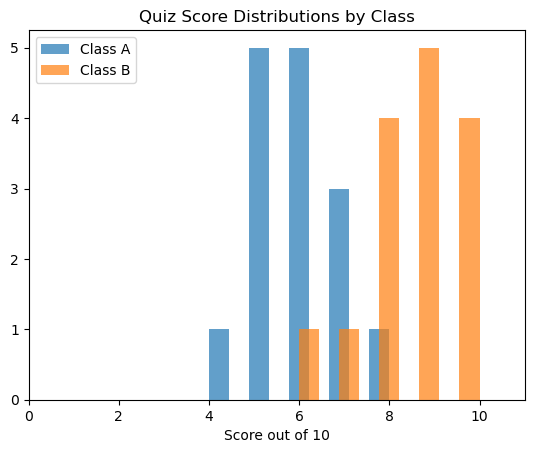
\includegraphics[width=0.4\textwidth]{img/dist_by_class.png}

\begin{lstlisting}
class_A = [5, 6, 5, 7, 6, 5, 8, 6, 7, 5, 4, 6, 7, 5, 6]
class_B = [9, 8, 10, 9, 10, 8, 9, 10, 6, 8, 9, 7, 8, 10, 9]

plt.boxplot(
    [class_A, class_B],
    labels=['Class A', 'Class B']
)

plt.title('Quiz Score Distributions by Class')
plt.show()
\end{lstlisting}
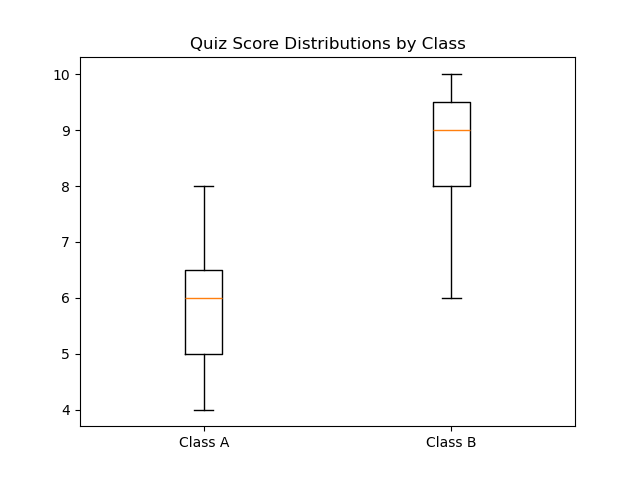
\includegraphics[width=0.45\textwidth]{img/boxwhisk.png}

There are many customizations that can be implemented for the plots above. See the matplotlib pyplot documentation.  

\end{multicols}
\end{document}
